\chapter{设计脚本语言}

\begin{flushleft}
故不登高山,不知天之高也;不临深溪,不知地之厚也;不闻先王之遗言,不知学问之大也。
\end{flushleft}

\begin{flushright}
---荀子   
\end{flushright}

\section{麻雀虽小五脏俱全}

设计脚本语言的基本元素如图2.1所示:

\begin{figure}[hbtp]
\centering
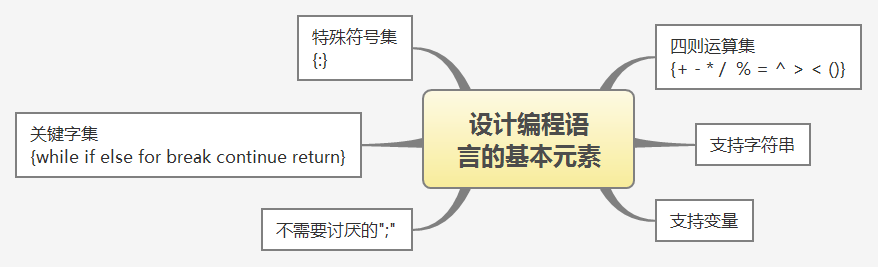
\includegraphics[width=1.0\textwidth]{pl.png}
\caption{脚本语言构成要素}
\end{figure}

只有具备这些基本元素才能算为一个完备的脚本语言,暂定这些基本元素,后期在有需要再进行进一
步的修改:
\begin{itemize}
	\item 支持四则运算
	\item 支持字符串
	\item 支持变量
	\item 一些其它特性,如不支持‘;’
	\item 支持基本逻辑关键字
\end{itemize}

